\documentclass[letter,11pt]{article}
%\documentclass[letter,twoside,11pt]{article}

\usepackage[spanish,es-nodecimaldot]{babel}
\usepackage[utf8]{inputenc}

\usepackage{lmodern}
\usepackage[T1]{fontenc}
\usepackage{textcomp}

\usepackage{framed}
\usepackage[svgnames]{xcolor}
\colorlet{shadecolor}{Gainsboro!50}

\usepackage{graphicx}
\usepackage{pstricks}

\usepackage{anysize}
\marginsize{3cm}{2cm}{2cm}{3cm}

\usepackage{amsmath}
\usepackage{array}
\usepackage{alltt}

\usepackage{fancyhdr}
\usepackage{lastpage}
\pagestyle{fancy}
\fancyhf{}
\fancyhead[LE,RO]{Laboratorio de Física Básica I}
\fancyfoot[CO,CE]{\thepage\ de \pageref{LastPage}}

\special{papersize=215.9mm,279.4mm}

\usepackage[
    pdfauthor={Carlos Eduardo Caballero Burgoa},%
    pdftitle={Laboratorio de Física Básica I},%
    pdfsubject={Dinámica: Segunda ley de Newton},%
    colorlinks,%
    citecolor=black,%
    filecolor=black,%
    linkcolor=black,%
    urlcolor=black,
    breaklinks]{hyperref}
\usepackage{breakurl}

\newcommand{\blankpage}{
\newpage
\thispagestyle{empty}
\mbox{}
\newpage
}

\renewcommand{\arraystretch}{1.2}

\begin{document}

\begin{titlepage}
\begin{center}
{\Large UNIVERSIDAD MAYOR DE SAN SIMÓN}\\
\vspace*{0.15cm}
{\large FACULTAD DE CIENCIAS Y TECNOLOGÍA}\\
\vspace*{0.10cm}
DEPARTAMENTO DE FÍSICA\\
\vspace*{3.0cm}
{\Large \textbf{LABORATORIO DE FÍSICA BÁSICA I}}\\
\vspace*{0.3cm}
{\Large \textbf{PRACTICA No. 7}}\\
\vspace*{3.5cm}
{\Large \textbf{DINÁMICA: SEGUNDA LEY DE NEWTON}}\\
\end{center}

\vspace*{7.4cm}
\leftskip=7.95cm
\noindent
\textbf{Estudiante:}\\
Caballero Burgoa, Carlos Eduardo.\\
\newline
\textbf{Docente:}\\
Msc. Guzmán Saavedra, Rocio.\\
\newline
\textbf{Grupo:} N5.\\
\textbf{Fecha de realización:} 11 de Enero del 2021.\\
\textbf{Fecha de entrega:} 11 de Enero del 2021.\\

\end{titlepage}

\blankpage

\section{Objetivo}
Comprobar la segunda ley de \emph{Newton}, a partir de las relación funcional:
Fuerza en función de la aceleración.

\section{Marco teórico}
La ecuación de \emph{Newton} para el movimiento rectilíneo de una masa puntual,
a la cual se aplica una fuerza $F$ es:

\begin{equation*}
    F = m a
\end{equation*}

\section{Materiales}
\begin{itemize}
\item Simulador «PhET Interactive Simulations» Fuerzas y movimiento.
\end{itemize}

\section{Procedimiento}
A continuación se describe el procedimiento experimental que se llevará a
cabo.

\begin{enumerate}
\item Haciendo uso del simulador, tomar datos de la aceleración $a$ resultante
    para diversas valores de fuerza $F$.
\item Graficar los datos tomados tal que pueda verse la relación funcional entre
    estas variables.
\item Hallar la ecuación de la recta por el método gráfico.
\item Aplicar el método de mínimos cuadrados, para hallar los coeficientes de la
    recta y sus errores.
\item Hallar la relación funcional de las variables e interpretar el significado
    físico del parámetro $B$ de la recta.
\end{enumerate}

\section{Tablas de datos y resultados}

\subsubsection{Datos obtenidos}

\begin{center}
\begin{tabular}{|c|>{\centering}m{2.25cm}<{\centering}
                  |>{\centering}m{2.25cm}<{\centering}|}
\hline
\multicolumn{3}{|c|}{\textbf{Tabla \#1: Aceleración-Fuerza}} \\
\hline
\multicolumn{3}{|c|}{Perro dormido $25 [kg]; \mu_c = \mu_e = 0.5$} \\
\hline
$i$ & $F_i [N]$ & $a_i [m/s^2]$ \tabularnewline \hline
  1 &  130 &  0.30 \tabularnewline \hline
  2 &  140 &  0.70 \tabularnewline \hline
  3 &  150 &  1.10 \tabularnewline \hline
  4 &  160 &  1.50 \tabularnewline \hline
  5 &  170 &  1.90 \tabularnewline \hline
  6 &  180 &  2.30 \tabularnewline \hline
  7 &  190 &  2.70 \tabularnewline \hline
  8 &  200 &  3.10 \tabularnewline \hline
  9 &  210 &  3.50 \tabularnewline \hline
 10 &  220 &  3.90 \tabularnewline \hline
 11 &  230 &  4.30 \tabularnewline \hline
 12 &  240 &  4.70 \tabularnewline \hline
 13 &  250 &  5.10 \tabularnewline \hline
 14 &  260 &  5.50 \tabularnewline \hline
 15 &  270 &  5.90 \tabularnewline \hline
 16 &  280 &  6.30 \tabularnewline \hline
 17 &  300 &  7.10 \tabularnewline \hline
 18 &  320 &  7.90 \tabularnewline \hline
 19 &  340 &  8.70 \tabularnewline \hline
 20 &  360 &  9.50 \tabularnewline \hline
 21 &  380 & 10.30 \tabularnewline \hline
 22 &  400 & 11.10 \tabularnewline \hline
 23 &  420 & 11.90 \tabularnewline \hline
 24 &  440 & 12.70 \tabularnewline \hline
 25 &  480 & 14.30 \tabularnewline \hline
 26 &  520 & 15.90 \tabularnewline \hline
 27 &  560 & 17.50 \tabularnewline \hline
 28 &  600 & 19.10 \tabularnewline \hline
 29 &  680 & 22.30 \tabularnewline \hline
 30 &  760 & 25.50 \tabularnewline \hline
 31 &  920 & 31.90 \tabularnewline \hline
 32 & 1240 & 44.70 \tabularnewline \hline
\end{tabular}
\quad
\begin{tabular}{|c|>{\centering}m{2.25cm}<{\centering}
                  |>{\centering}m{2.25cm}<{\centering}|}
\hline
\multicolumn{3}{|c|}{\textbf{Tabla \#2: Aceleración-Fuerza}} \\
\hline
\multicolumn{3}{|c|}{Objeto misterioso} \\
\hline
$i$ & $F_i [N]$ & $a_i [m/s^2]$ \tabularnewline \hline
  1 &  130 & 0    \tabularnewline \hline
  2 &  140 & 0    \tabularnewline \hline
  3 &  150 & 0    \tabularnewline \hline
  4 &  160 & 0    \tabularnewline \hline
  5 &  170 & 0    \tabularnewline \hline
  6 &  180 & 0    \tabularnewline \hline
  7 &  190 & 0    \tabularnewline \hline
  8 &  200 & 0    \tabularnewline \hline
  9 &  210 & 0    \tabularnewline \hline
 10 &  220 & 0    \tabularnewline \hline
 11 &  230 & 0    \tabularnewline \hline
 12 &  240 & 0    \tabularnewline \hline
 13 &  250 & 0.07 \tabularnewline \hline
 14 &  260 & 0.15 \tabularnewline \hline
 15 &  270 & 0.24 \tabularnewline \hline
 16 &  280 & 0.32 \tabularnewline \hline
 17 &  300 & 0.48 \tabularnewline \hline
 18 &  320 & 0.64 \tabularnewline \hline
 19 &  340 & 0.80 \tabularnewline \hline
 20 &  360 & 0.97 \tabularnewline \hline
 21 &  380 & 1.13 \tabularnewline \hline
 22 &  400 & 1.29 \tabularnewline \hline
 23 &  420 & 1.45 \tabularnewline \hline
 24 &  440 & 1.62 \tabularnewline \hline
 25 &  480 & 1.94 \tabularnewline \hline
 26 &  520 & 2.27 \tabularnewline \hline
 27 &  560 & 2.56 \tabularnewline \hline
 28 &  600 & 2.92 \tabularnewline \hline
 29 &  680 & 3.57 \tabularnewline \hline
 30 &  760 & 4.22 \tabularnewline \hline
 31 &  920 & 5.52 \tabularnewline \hline
 32 & 1240 & 8.12 \tabularnewline \hline
\end{tabular}
\end{center}

\section{Gráficas}

\subsection{Perro dormido $m = 25 [kg]$}
Para la tabla \#1 se tiene:

\begin{figure}[!h]
\centering
\includegraphics[scale=1.00]{resources/7.1.1.eps}
\caption{Gráfica de aceleración en función de la fuerza}
\label{practica71}
\end{figure}

Por la forma de la figura \ref{practica71} el modelo que se asume para la
relación funcional $a = a(F)$ es:

\begin{equation*}
    a = A + B F
\end{equation*}

\subsubsection{Método de mínimos cuadrados}

Calculando los valores de la recta por el método de los mínimos cuadrados, se
obtiene:

\begin{equation*}
    A = (-4.9 \pm 0.0)[m/s^2];0\%
\end{equation*}

\begin{equation*}
    B = (0.04 \pm 0.0)[kg^{-1}];0\%
\end{equation*}

Con los parámetros obtenidos la relación $a = a(F)$ es:

\begin{equation}
    a = - 4.9 + 0.04 F
\end{equation}

Siendo la relación funcional:

\begin{equation}
    a = \frac{1}{25} F
\end{equation}

El significado físico del parámetro $B = 0.04$ es el valor inverso de la masa,
debido a que $F$ es la variable independiente y $a$ la variable dependiente.

\subsubsection{Memoria de calculo}

\begin{shaded}
\begin{alltt}
\footnotesize
\# Entrada del programa:
\input{resources/i7_1.csv}

\# Comandos del programa:
\input{resources/p7_1_2.m}

\# Salida del programa
\input{resources/o7_1_2.txt}
\normalsize
\end{alltt}
\end{shaded}

\subsection{Objeto misterioso}
Para la tabla \#2 se tiene:

\begin{figure}[!h]
\centering
\includegraphics[scale=1.00]{resources/7.2.1.eps}
\caption{Gráfica de aceleración en función de la fuerza}
\label{practica73}
\end{figure}

Por la forma de la figura \ref{practica73} el modelo que se asume para la
relación funcional $a = a(F)$ es:

\begin{equation*}
    a = A + B F
\end{equation*}

\subsubsection{Método de mínimos cuadrados}

Calculando los valores de la recta por el método de los mínimos cuadrados, se
obtiene:

\begin{equation*}
    A = (-1.961 \pm 0.004)[m/s^2];0.20\%
\end{equation*}

\begin{equation*}
    B = (0.0081 \pm 0.000007)[kg^{-1}];0.09\%
\end{equation*}

Con los parámetros obtenidos la relación $a = a(F)$ es:

\begin{equation}
    a = - 1.961 + 0.0081 F
\end{equation}

Siendo la relación funcional:

\begin{equation}
    a = \frac{1}{123.46} F
\end{equation}

El significado físico del parámetro $B = 0.008$ es el valor inverso de la masa,
debido a que $F$ es la variable independiente y $a$ la variable dependiente.

\subsubsection{Memoria de calculo}

\begin{shaded}
\begin{alltt}
\footnotesize
\# Entrada del programa:
\input{resources/i7_2.csv}

\# Comandos del programa:
\input{resources/p7_2_2.m}

\# Salida del programa
\input{resources/o7_2_2.txt}
\normalsize
\end{alltt}
\end{shaded}

\section{Cuestionario}
\begin{enumerate}
\item \textbf{¿Qué tipo de relación existe entre la aceleración y el inverso de
    la masa del sistema?}

La relación entre la aceleración y el inverso de la masa es una relación lineal

\begin{equation*}
    a \propto \frac{1}{m}
\end{equation*}

\item \textbf{¿Se verifica la segunda ley de \emph{Newton}?}

La segunda ley de \emph{Newton} esta verificada, ya que la constante de
proporcionalidad en la relación $a = a(F)$, es el inverso de la masa, y por
ende:

\begin{equation*}
    a = \frac{1}{m} F
\end{equation*}

\end{enumerate}

\end{document}

